\section{Technical Architecture}


\subsection{System Components}

Lux.id architecture consists of:

\begin{figure}[h]
\centering
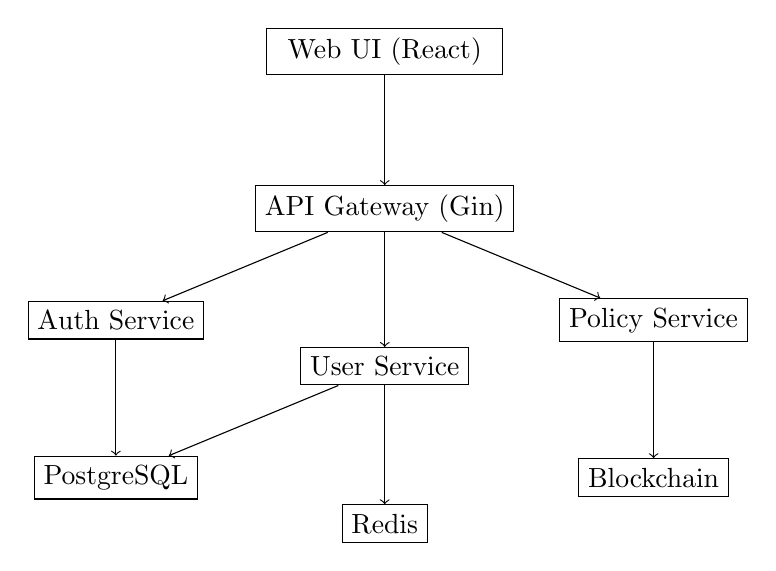
\begin{tikzpicture}[node distance=2cm, auto]
    % Frontend
    \node[rectangle, draw, minimum width=3cm] (ui) {Web UI (React)};

    % API Gateway
    \node[rectangle, draw, minimum width=3cm, below of=ui] (api) {API Gateway (Gin)};

    % Core Services
    \node[rectangle, draw, below left of=api, xshift=-2cm] (auth) {Auth Service};
    \node[rectangle, draw, below of=api] (user) {User Service};
    \node[rectangle, draw, below right of=api, xshift=2cm] (policy) {Policy Service};

    % Data Layer
    \node[rectangle, draw, below of=auth] (postgres) {PostgreSQL};
    \node[rectangle, draw, below of=user] (redis) {Redis};
    \node[rectangle, draw, below of=policy] (chain) {Blockchain};

    % Connections
    \draw[->] (ui) -- (api);
    \draw[->] (api) -- (auth);
    \draw[->] (api) -- (user);
    \draw[->] (api) -- (policy);
    \draw[->] (auth) -- (postgres);
    \draw[->] (user) -- (postgres);
    \draw[->] (user) -- (redis);
    \draw[->] (policy) -- (chain);
\end{tikzpicture}
\caption{Lux.id System Architecture}
\end{figure}

\subsection{Backend Implementation}

The Go backend uses:

\begin{itemize}
    \item \textbf{Gin Framework}: High-performance HTTP router
    \item \textbf{GORM}: Object-relational mapping
    \item \textbf{go-redis}: Redis client for session management
    \item \textbf{jwt-go}: JWT token generation and validation
    \item \textbf{crypto/ecdsa}: Elliptic curve cryptography
\end{itemize}

\subsection{Database Schema}

Core tables structure:

\begin{lstlisting}[language=SQL]
CREATE TABLE users (
    id VARCHAR(255) PRIMARY KEY,
    owner VARCHAR(100),
    name VARCHAR(100),
    email VARCHAR(100),
    password_hash VARCHAR(100),
    wallet_address VARCHAR(42),
    did VARCHAR(255),
    created_time TIMESTAMP,
    updated_time TIMESTAMP
);

CREATE TABLE sessions (
    id VARCHAR(255) PRIMARY KEY,
    user_id VARCHAR(255),
    token VARCHAR(500),
    expires_at TIMESTAMP,
    ip_address VARCHAR(45),
    user_agent TEXT
);

CREATE TABLE permissions (
    id VARCHAR(255) PRIMARY KEY,
    role_id VARCHAR(255),
    resource VARCHAR(255),
    action VARCHAR(50),
    effect VARCHAR(10)
);
\end{lstlisting}

\subsection{Caching Strategy}

Redis caching for performance:

\begin{lstlisting}[language=C]
type CacheManager struct {
    client *redis.Client
    ttl    time.Duration
}

func (c *CacheManager) GetUser(id string) (*User, error) {
    key := fmt.Sprintf("user:%s", id)

    // Try cache first
    val, err := c.client.Get(ctx, key).Result()
    if err == nil {
        var user User
        json.Unmarshal([]byte(val), &user)
        return &user, nil
    }

    // Fetch from database
    user := fetchUserFromDB(id)

    // Update cache
    data, _ := json.Marshal(user)
    c.client.Set(ctx, key, data, c.ttl)

    return user, nil
}
\end{lstlisting}

\subsection{API Design}

RESTful API following OpenAPI 3.0:

\begin{lstlisting}[language=yaml]
/api/v1/users:
  get:
    summary: List users
    parameters:
      - name: limit
        in: query
        schema:
          type: integer
      - name: offset
        in: query
        schema:
          type: integer
    responses:
      200:
        description: User list
        content:
          application/json:
            schema:
              type: array
              items:
                $ref: '#/components/schemas/User'
\end{lstlisting}

